\documentclass[journal,12pt,twocolumn]{IEEEtran}
\usepackage{setspace}
\usepackage{gensymb}
\usepackage{xcolor}
\usepackage{caption}
%\usepackage{subcaption}
%\doublespacing
\singlespacing
%\usepackage{graphicx}
%\usepackage{amssymb}
%\usepackage{relsize}
\usepackage[cmex10]{amsmath}
\usepackage{mathtools}
%\usepackage{amsthm}
%\interdisplaylinepenalty=2500
%\savesymbol{iint}
%\usepackage{txfonts}
%\restoresymbol{TXF}{iint}
%\usepackage{wasysym}
\usepackage{hyperref}
\usepackage{amsthm}
\usepackage{mathrsfs}
\usepackage{txfonts}
\usepackage{stfloats}
\usepackage{cite}
\usepackage{cases}
\usepackage{subfig}
%\usepackage{xtab}
\usepackage{longtable}
\usepackage{multirow}
%\usepackage{algorithm}
%\usepackage{algpseudocode}
%\usepackage{enumerate}
\usepackage{enumitem}
\usepackage{mathtools}
%\usepackage{iithtlc}
%\usepackage[framemethod=tikz]{mdframed}
\usepackage{listings}
\usepackage{scalerel}
\usepackage{siunitx}
\setcounter{MaxMatrixCols}{20}

\newcommand{\longdiv}{\smash{\mkern-0.43mu\vstretch{1.31}{\hstretch{.7}{)}}\mkern-5.2mu\vstretch{1.31}{\hstretch{.7}{)}}}}
\newcommand{\myvec}[1]{\ensuremath{\begin{pmatrix}#1\end{pmatrix}}}
\newcommand{\mydet}[1]{\ensuremath{\begin{vmatrix}#1\end{vmatrix}}}
\newcommand{\define}{\stackrel{\triangle}{=}}
\newcommand{\mymat}[1]{\ensuremath{\begin{bmatrix}#1\end{bmatrix}}}

%\usepackage{wasysym}
%\newcounter{MYtempeqncnt}
\DeclareMathOperator*{\Res}{Res}
%\renewcommand{\baselinestretch}{2}
\renewcommand\thesection{\arabic{section}}
\renewcommand\thesubsection{\thesection.\arabic{subsection}}
\renewcommand\thesubsubsection{\thesubsection.\arabic{subsubsection}}

\renewcommand\thesectiondis{\arabic{section}}
\renewcommand\thesubsectiondis{\thesectiondis.\arabic{subsection}}
\renewcommand\thesubsubsectiondis{\thesubsectiondis.\arabic{subsubsection}}

%\renewcommand{\labelenumi}{\textbf{\theenumi}}
%\renewcommand{\theenumi}{P.\arabic{enumi}}

% correct bad hyphenation here
\hyphenation{op-tical net-works semi-conduc-tor}

\lstset{
language=Python,
frame=single, 
breaklines=true,
columns=fullflexible
}

\begin{document}

\theoremstyle{definition}
\newtheorem{theorem}{Theorem}[section]
\newtheorem{problem}{Problem}
\newtheorem{proposition}{Proposition}[section]
\newtheorem{lemma}{Lemma}[section]
\newtheorem{corollary}[theorem]{Corollary}
\newtheorem{example}{Example}[section]
\newtheorem{definition}{Definition}[section]
%\newtheorem{algorithm}{Algorithm}[section]
%\newtheorem{cor}{Corollary}
\newcommand{\BEQA}{\begin{eqnarray}}
\newcommand{\EEQA}{\end{eqnarray}}
% \newcommand{\define}{\stackrel{\triangle}{=}}

\bibliographystyle{IEEEtran}
%\bibliographystyle{ieeetr}

\providecommand{\nCr}[2]{\,^{#1}C_{#2}} % nCr
\providecommand{\nPr}[2]{\,^{#1}P_{#2}} % nPr
\providecommand{\mbf}{\mathbf}
\providecommand{\pr}[1]{\ensuremath{\Pr\left(#1\right)}}
\providecommand{\qfunc}[1]{\ensuremath{Q\left(#1\right)}}
\providecommand{\sbrak}[1]{\ensuremath{{}\left[#1\right]}}
\providecommand{\lsbrak}[1]{\ensuremath{{}\left[#1\right.}}
\providecommand{\rsbrak}[1]{\ensuremath{{}\left.#1\right]}}
\providecommand{\brak}[1]{\ensuremath{\left(#1\right)}}
\providecommand{\lbrak}[1]{\ensuremath{\left(#1\right.}}
\providecommand{\rbrak}[1]{\ensuremath{\left.#1\right)}}
\providecommand{\cbrak}[1]{\ensuremath{\left\{#1\right\}}}
\providecommand{\lcbrak}[1]{\ensuremath{\left\{#1\right.}}
\providecommand{\rcbrak}[1]{\ensuremath{\left.#1\right\}}}
\theoremstyle{remark}
\newtheorem{rem}{Remark}
\newcommand{\sgn}{\mathop{\mathrm{sgn}}}
\providecommand{\abs}[1]{\left\vert#1\right\vert}
\providecommand{\res}[1]{\Res\displaylimits_{#1}} 
\providecommand{\norm}[1]{\lVert#1\rVert}
\providecommand{\mtx}[1]{\mathbf{#1}}
\providecommand{\mean}[1]{E\left[ #1 \right]}
\providecommand{\fourier}{\overset{\mathcal{F}}{ \rightleftharpoons}}
\providecommand{\ztrans}{\overset{\mathcal{Z}}{ \rightleftharpoons}}

%\providecommand{\hilbert}{\overset{\mathcal{H}}{ \rightleftharpoons}}
\providecommand{\system}{\overset{\mathcal{H}}{ \longleftrightarrow}}
	%\newcommand{\solution}[2]{\textbf{Solution:}{#1}}
\newcommand{\solution}{\noindent \textbf{Solution: }}
\providecommand{\dec}[2]{\ensuremath{\overset{#1}{\underset{#2}{\gtrless}}}}
\numberwithin{equation}{section}
%\numberwithin{equation}{subsection}
%\numberwithin{problem}{subsection}
%\numberwithin{definition}{subsection}
\makeatletter
\@addtoreset{figure}{problem}
\makeatother
\let\vec\mathbf

\let\StandardTheFigure\thefigure
%\renewcommand{\thefigure}{\theproblem.\arabic{figure}}
\renewcommand{\thefigure}{\theproblem}


%\numberwithin{figure}{subsection}

\def\putbox#1#2#3{\makebox[0in][l]{\makebox[#1][l]{}\raisebox{\baselineskip}[0in][0in]{\raisebox{#2}[0in][0in]{#3}}}}
     \def\rightbox#1{\makebox[0in][r]{#1}}
     \def\centbox#1{\makebox[0in]{#1}}
     \def\topbox#1{\raisebox{-\baselineskip}[0in][0in]{#1}}
     \def\midbox#1{\raisebox{-0.5\baselineskip}[0in][0in]{#1}}

\vspace{3cm}

\title{Digital Signal Processing}

\author{Donal Loitam} 

% make the title area
\maketitle

%\newpage

\tableofcontents

%\renewcommand{\thefigure}{\thesection.\theenumi}
%\renewcommand{\thetable}{\thesection.\theenumi}

\renewcommand{\thefigure}{\theenumi}
\renewcommand{\thetable}{\theenumi}

%\renewcommand{\theequation}{\thesection}


\bigskip

\begin{abstract}
This manual provides a simple introduction to digital signal processing.
\end{abstract}
\noindent \section{Software Installation}
\noindent Run the following commands
\begin{lstlisting}
 sudo apt -get update 
 sudo apt install libffi-dev libsndfile1 python3-scipy python3-numpy python3-matplotlib 
sudo pip install cffi pysoundfile 
\end{lstlisting}
\section{Digital Filter}
\begin{enumerate}[label=\thesection.\arabic*
,ref=\thesection.\theenumi]
\item
\label{prob:input}
Download the sound file using
\begin{lstlisting}
 wget https://github.com/Donal-08/EE3900-assignments/blob/main/Assignment_1/codes/Sound_Noise.wav
\end{lstlisting}
\item
\label{prob:spectrogram}
You will find a spectrogram at \href{https://academo.org/demos/spectrum-analyzer}{\url{https://academo.org/demos/spectrum-analyzer}}. Upload the sound file that you downloaded in Problem \ref{prob:input} in the spectrogram and play. Observe the spectrogram. What do you find?

\solution There are a lot of yellow lines between 440 Hz to 5.1 KHz.  These represent the synthesizer key tones. Also, the key strokes
are audible along with background noise.
\item
\label{prob:output}
Write the python code for removal of out of band noise and execute the code.

\solution
Download the source code using
\begin{lstlisting}
 wget https://github.com/Donal-08/EE3900-assignments/blob/main/Assignment_1/codes/2_3.py_
\end{lstlisting}
and execute it using
\begin{lstlisting}
$ python3 2_3.py
\end{lstlisting}
\item
The output of the python script in Problem \ref{prob:output} is the audio file \texttt{Sound\_With\_ReducedNoise.wav}. Play the file in the spectrogram in Problem \ref{prob:spectrogram}. What do you observe?

\solution The key strokes as well as background noise is subdued in the audio. Also, the signal is blank for frequencies above 5.1 kHz.

\end{enumerate}
\section{Difference Equation}
\begin{enumerate}[label=\thesection.\arabic*,ref=\thesection.\theenumi]
\item Let
\begin{equation}
x(n) = \cbrak{\underset{\uparrow}{1},2,3,4,2,1}
\end{equation}
Sketch $x(n)$.
\item Let
\begin{multline}
\label{eq:iir_filter}
y(n) + \frac{1}{2}y(n-1) = x(n) + x(n-2), 
\\
y(n) = 0, n < 0
\end{multline}
Sketch $y(n)$.

\solution The following code yields Fig. \eqref{fig:xnyn}.
\begin{lstlisting}
 wget https://github.com/Donal-08/EE3900-assignments/blob/main/Assignment_1/codes/3_2.py
\end{lstlisting}
and execute it using
\begin{lstlisting}
$ python3 3_2.py
\end{lstlisting}

\begin{figure}[!ht]
	\centering
	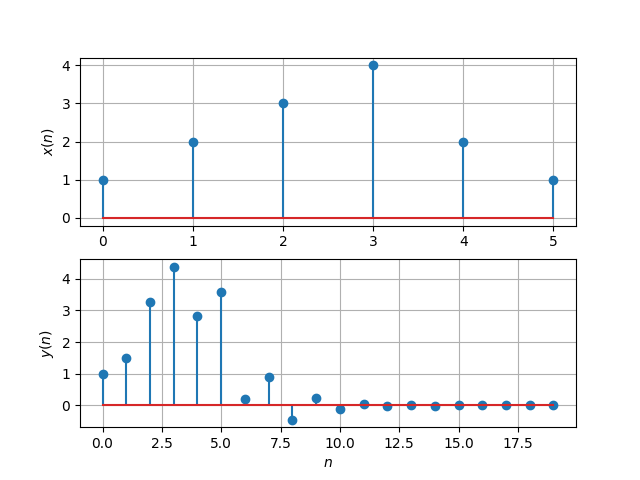
\includegraphics[width=\columnwidth]{figs/3_2.png}
	\caption{Plot of $x(n)$ and $y(n)$}
	\label{fig:xnyn}
\end{figure}
\item Repeat the above exercise using C code. \\
 \solution The following code yields Fig. \eqref{fig:xnyn}.
\begin{lstlisting}
 wget https://github.com/Donal-08/EE3900-assignments/blob/main/Assignment_1/codes/3_2.py
 wget https://github.com/Donal-08/EE3900-assignments/blob/main/Assignment_1/codes/3_2.c
\end{lstlisting}
\end{enumerate}

\section{$Z$-transform}
\begin{enumerate}[label=\thesection.\arabic*]
\item The $Z$-transform of $x(n)$ is defined as
\begin{equation}
\label{eq:z_trans}
X(z)={\mathcal {Z}}\{x(n)\}=\sum _{n=-\infty }^{\infty }x(n)z^{-n}
\end{equation}
Show that
\begin{equation}
\label{eq:shift1}
{\mathcal {Z}}\{x(n-1)\} = z^{-1}X(z)
\end{equation}
and find
\begin{equation}
	{\mathcal {Z}}\{x(n-k)\} 
\end{equation}
\solution From \eqref{eq:z_trans},
\begin{align}
{\mathcal {Z}}\{x(n-k)\} &=\sum _{n=-\infty }^{\infty }x(n-k)z^{-n}\\
&=\sum _{n=-\infty }^{\infty }x(n)z^{-n-k} \\
&= z^{-k}\sum _{n=-\infty }^{\infty }x(n)z^{-n} \\
&= z^{-k}X\brak{n}
\label{eq:z_trans_shift}
\end{align}
Putting $k = 1$ gives \eqref{eq:shift1}. or
\begin{align}
	{\mathcal {Z}}\{x(n-1)\} =  z^{-1}X(z)
\end{align}
\item Obtain $X(z)$ for $x(n)$ defined in problem 
	3.1 \\
\solution For the given $x(n)$, we have
\begin{align}
	\mathcal{Z} \cbrak{x(n)} &= \sum_{n=0}^5x(n)z^{-n} \\
	X(z) &= 1 + 2z^{-1} + 3z^{-2} + 4z^{-3} \nonumber \\
		&+ 2z^{-4} + z^{-5} \\
	\implies {\mathcal {Z}}\{x(n-1)\} &= z^{-1} + 2z^{-2} + 3z^{-3} \nonumber \\
									  &+4z^{-4} + 2z^{-5} + z^{-6} \\
	&= z^{-1}X(z)
\end{align}	
which also proves \ref{eq:z_trans_shift}
\item Find
\begin{equation}
H(z) = \frac{Y(z)}{X(z)}
\end{equation}
from  \eqref{eq:iir_filter} assuming that the $Z$-transform is a linear operation.

\solution  Applying \eqref{eq:z_trans_shift} in \eqref{eq:iir_filter},
\begin{align}
Y(z) + \frac{1}{2}z^{-1}Y(z) &= X(z)+z^{-2}X(z) \\
\implies \frac{Y(z)}{X(z)} &= \frac{1 + z^{-2}}{1 + \frac{1}{2}z^{-1}}
\label{eq:freq_resp}
\end{align}

\item Find the Z transform of 
\begin{equation}
\delta(n) =
\begin{cases}
1 & n = 0 \\
0 & \text{otherwise}
\end{cases}
\label{eq:dirac-delta}
\end{equation}
and show that the $Z$-transform of
\begin{equation}
\label{eq:unit_step}
u(n) =
\begin{cases}
1 & n \ge 0 \\
0 & \text{otherwise}
\end{cases}
\end{equation}
is
\begin{equation}
U(z) = \frac{1}{1-z^{-1}}, \quad \abs{z} > 1
\end{equation}
\solution We see using \eqref{eq:dirac-delta} that
\begin{align}
	\mathcal{Z}\cbrak{\delta\brak{n}} &= \sum_{n=\infty}^{\infty} \delta(n)z^{-n} = \delta\brak{0}z^{0} \\
	&=	\delta\brak{0} = 1	
\end{align}
and from \eqref{eq:unit_step},
\begin{align}
U(z) &= \sum _{n= 0}^{\infty}z^{-n} \\
&=\frac{1}{1-z^{-1}}, \quad \abs{z} > 1
\end{align}
using the fomula for the sum of an infinite geometric progression.

\item Show that 
\begin{equation}
\label{eq:anun}
a^nu(n) \ztrans \frac{1}{1-az^{-1}} \quad \abs{z} > \abs{a}
\end{equation}

\solution
\begin{align}
	a^nu(n) &\ztrans \sum_{n = 0}^{\infty}\brak{az^{-1}}^n \\
			&= \frac{1}{1-az^{-1}} \quad \abs{z} > \abs{a}
\end{align}

\item 
Let
\begin{equation}
H\brak{e^{\j \omega}} = H\brak{z = e^{\j \omega}}.
\end{equation}
Plot $\abs{H\brak{e^{\j \omega}}}$.  Comment.  $H(e^{\j \omega})$ is
known as the {\em Discret Time Fourier Transform} (DTFT) of $x(n)$.

\solution The following code plots Fig. \eqref{fig:H-w}.
\begin{lstlisting}
	wget https://github.com/Donal-08/EE3900-assignments/blob/main/Assignment_1/codes/4_5.py
\end{lstlisting}
The figure can be generated using
\begin{lstlisting}
$ python3 4_5.py
\end{lstlisting}
Using \eqref{eq:freq_resp}, we observe that $\left|H\brak{e^{\j\omega}}\right|$ is given by
\begin{align}
	\left|H\brak{e^{\j\omega}}\right| &= \left|\frac{1 + e^{-2\j\omega}}{1 + \frac{1}{2}e^{-\j\omega}}\right| \\
									  &= \sqrt{\frac{\brak{1 + \cos{2\omega}}^2 + \brak{\sin{2\omega}}^2}{\brak{1 + \frac{1}{2}\cos{\omega}}^2 + \brak{\frac{1}{2}\sin{\omega}}^2}}\\
									  &= \sqrt{\frac{2\brak{1 + \cos{2\omega}}}{\frac{5}{4} + \cos{\omega}}} \\
									  &= \sqrt{\frac{2\brak{2\cos^2{\omega}}}{\frac{5}{4} + \cos{\omega}}} \\
									  &= \frac{4|\cos{\omega}|}{\sqrt{5 + 4\cos{\omega}}}
\end{align}
Now , we know that a function is periodic with period T if $f(t+T)=f(t),$ $\forall t \in D$ where D = Domain of $f(t)$
\begin{align}
	\left|cos(\omega+\pi)\right| &= \left|-cos(\omega)\right| = \left|cos(\omega)\right| \\
	& cos\brak{\omega+2\pi} = cos(\omega) \\
	& L.C.M(2\pi, \pi) =  2\pi
\end{align}
Clearly the L.C.M of the fundamnetal period of numerator and denomintor  is $2\pi$
and so its fundamental period is $2\pi$.
\begin{figure}[!ht]
	\centering
	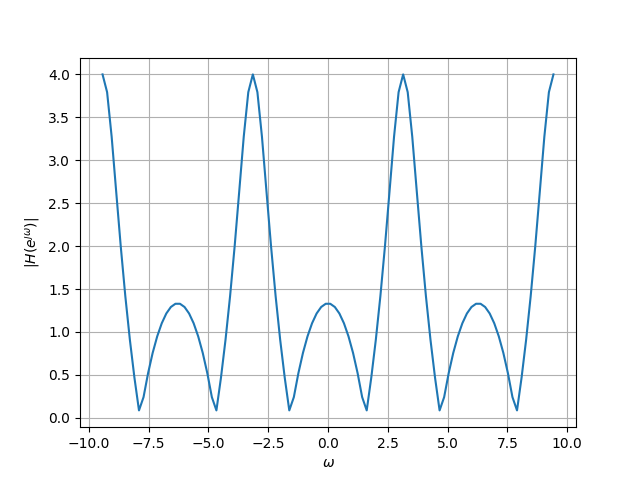
\includegraphics[width=\columnwidth]{figs/4_5.png}
	\caption{Plot of $\left|H\brak{e^{j\omega}}\right|$ against $\omega$}
	\label{fig:H-w}
\end{figure}
\item Express $h(n)$ in terms of $H(e^{\j\omega})$. \\

\solution Given 
\begin{align}
	H(e^{j\omega}) &= \sum_{n=-\infty}^{\infty} h(n)e^{-j\omega n} 
\end{align}
We can prove the IDFT equation as follows :
\begin{align}
	&\int_{-\pi}^{\pi}H(e^{-j\omega})e^{j\omega k}d\omega \\
	&= \sum_{n=-\infty}^{\infty} h(n)\int_{-\pi}^{\pi} e^{-j\omega n}e^{j\omega k} d\omega \\
	   &= \begin{cases}
		0 \hspace{20mm} \text{if  } n \neq k\\
		 h(n)\int_{-\pi}^{\pi} e^{-j\omega (n - n)} d\omega \hspace{5mm}  {,n=k} \\
	  \end{cases} \\
	  &\text{i.e  } \int_{-\pi}^{\pi}H(e^{-j\omega})e^{j\omega k}d\omega = h(n)  (2\pi) 
\end{align}
\begin{align}
	\therefore h(n) &= \frac{1}{2\pi}\int_{-\pi}^{\pi}H(e^{\j\omega})e^{\j\omega n}d\omega 
\end{align}
\end{enumerate}

\section{Impulse Response}
\begin{enumerate}[label=\thesection.\arabic*]
\item Using long division, find
\begin{align}
	h(n), \quad n < 5
\end{align}
\solution \begin{align}
	H(z) = \frac{1+z^{-2}}{1+\frac{1}{2}z^{-1}}
\end{align}
Substitute $z^{-1} = x$ for simplicity
\[
\arraycolsep=1pt
\renewcommand\arraystretch{1.2}
\begin{array}{*1r @{\hskip\arraycolsep}c@{\hskip\arraycolsep} *{11}r}
        &          & 2x & - & 4  \\
\cline{2-13}
1+\frac{x}{2} & \longdiv & x^2 & +  & 1  &   &      &   &      &   &      &   &        \\
        &          & - & x^2 & - & 2x &   &   &      &   &      &   &        \\
\cline{3-7}
        &          &   &   & - & 2x & + &  1 &      &   &      &   &        \\
        &          &   &   &  & 2x &  + & 4 &   &   &      &   &        \\
\cline{5-9}
        &          &   &   &   &   &  & 5 &   &   &      &   &        \\
\end{array}
\]
\begin{align}
	&\implies 1 + z^{-2} = \brak{1+\frac{1}{2}z^{-1}}(-4+2z^{-1}) + 5\\
	&\implies H(z) = -4+2z^{-1} + \frac{5}{1+\frac{1}{2}z^{-1}}
\end{align}


\begin{align}
	\frac{5}{1 + \frac12 z^{-1}} &= 5 \brak{1 + \frac12 z^{-1}}^{-1} \\
	&= 5 \sum_{n=0}^\infty \brak{-\frac{z^{-1}}{2}}^n
\end{align}

\begin{multline}
	H(z) = -4 + 2z^{-1} + 5 - \frac{5}{2}z^{-1} + \frac{5}{4}z^{-2}\\ - \frac{5}{8}z^{-3}  + \frac{5}{16}z^{-4} - \frac{5}{32}z^{-5} + \cdots
\end{multline}

Therefore, by comparing coefficients
\begin{align}
	h(n) = 
	\begin{cases}
		1 & n = 0 \\
		-\dfrac12 & n = 1 \\
		\dfrac{5}{4} & n = 2 \\
		-\dfrac{5}{8} & n = 3 \\
		\dfrac{5}{16} & n = 4 \\
	\end{cases}
\end{align}

Alternatively, on applying the inverse $Z$-transform on both sides of the equation
\begin{align}
	H(z) &\ztrans h(n) \\
	-4 &\ztrans -4\delta(n) \\
	2z^{-1} &\ztrans 2\delta(n - 1) \\
	\frac{5}{1 + \frac12 z^{-1}} &\ztrans 5\brak{-\frac12}^n u(n) \\
\end{align}

Therefore,
\begin{equation}
	h(n) = -4\delta(n) + 2\delta(n - 1) + 5\brak{-\frac12}^n u(n)
\end{equation}

Download the following Python code that plots Fig. \ref{fig-5.1}.
\begin{lstlisting}
	wget https://github.com/Donal-08/EE3900-assignments/tree/main/Assignment_1/codes/5_1.py
\end{lstlisting}

Run the code by executing
\begin{lstlisting}
	python 5.1.py
\end{lstlisting}

\begin{figure}[!ht]
	\centering
	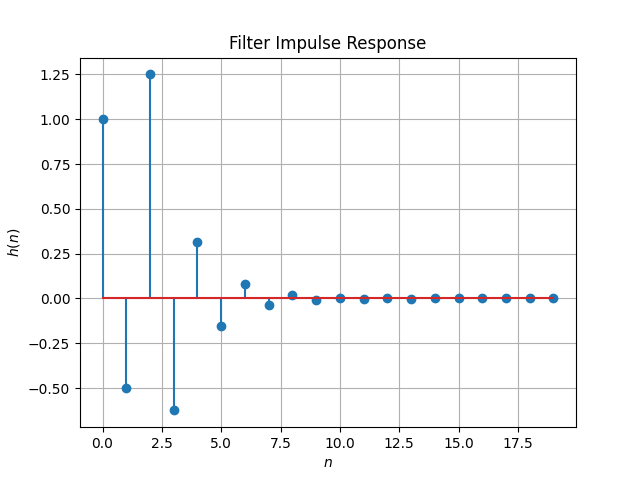
\includegraphics[width=\columnwidth]{./figs/5.1.png}
	\caption{Plot of $h(n)$}
	\label{fig-5.1}	
\end{figure} 
\item \label{prob:impulse_resp}
Find an expression for $h(n)$ using $H(z)$, given that 
\begin{equation}
\label{eq:impulse_resp}
h(n) \ztrans H(z)
\end{equation}
and there is a one to one relationship between $h(n)$ and $H(z)$. $h(n)$ is known as the {\em impulse response} of the
system defined by \eqref{eq:iir_filter}.

\solution From \eqref{eq:freq_resp},
\begin{align}
H(z) &= \frac{1}{1 + \frac{1}{2}z^{-1}} + \frac{ z^{-2}}{1 + \frac{1}{2}z^{-1}} \\
\implies h(n) &= \brak{-\frac{1}{2}}^{n}u(n) + \brak{-\frac{1}{2}}^{n-2}u(n-2)
\end{align}
using \eqref{eq:anun} and \eqref{eq:z_trans_shift}.
\begin{align}
	a^nu(n) \ztrans \frac{1}{1-az^{-1}} \quad \abs{z} > \abs{a}
\end{align}
Since Z-transform is a linear operator 

\item Sketch $h(n)$. Is it bounded? Convergent? 

\solution The following code plots Fig. \eqref{fig:h-n}.
\begin{lstlisting}
$ wget https://github.com/Donal-08/EE3900-assignments/blob/main/Assignment_1/codes/5_2.py
\end{lstlisting}
and execute it using
\begin{lstlisting}
$ python3 5_2.py
\end{lstlisting}

\begin{figure}[!ht]
	\centering
	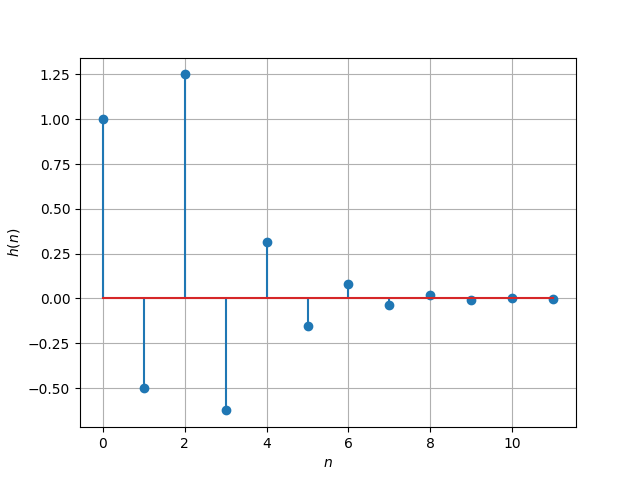
\includegraphics[width=\columnwidth]{figs/5_2.png}
	\caption{$h(n)$ as the inverse of $H(z)$}
	\label{fig:h-n}
\end{figure}
Theoretically,
	\begin{align}
		\abs{u(n)} &\le 1 \\
		\abs{\brak{-\frac12}^n} &\le 1 \\
		\implies \abs{\brak{-\frac12}^n u(n)} &\le 1
	\end{align}
	
	Similarly,
	\begin{align}
		\abs{\brak{-\frac12}^{n-2} u(n-2)} &\le 1 \\
		\implies h(n) &\le 2
	\end{align}
	
	Therefore $h(n)$ is bounded. 
	\item Is it convergent? Justify using the ratio test.
	\solution $h(n)$ is also convergent. For large $n$, $u(n)=1$ and so,
\begin{align}
	h(n) &= \brak{-\frac{1}{2}}^n + \brak{-\frac{1}{2}}^{n - 2} \\
		 &= \brak{-\frac{1}{2}}^{n}\brak{4 + 1} = 5\brak{-\frac{1}{2}}^n \\
		 &\implies \left|\frac{h(n + 1)}{h(n)}\right| = \frac{1}{2}\\
		 &\text{i.e  } \lim_{n \to \infty}\left|\frac{h(n + 1)}{h(n)}\right| = \frac{1}{2} < 1
\end{align}
and since, $\lim_{n \to \infty}\left|\frac{h(n + 1)}{h(n)}\right| = \frac{1}{2} < 1$,we can conclude by \textit{Ratio Test} that $h(n)$ converges. 

\item The system with $h(n)$ is defined to be stable if
\begin{equation}
\sum_{n=-\infty}^{\infty}h(n) < \infty
\end{equation}
Is the system defined by \eqref{eq:iir_filter} stable for the impulse response in \eqref{eq:impulse_resp}?

\solution
Note that
\begin{align}
	\sum_{n = -\infty}^{\infty}h\brak{n} &= \sum_{n = -\infty}^{\infty}\brak{-\frac{1}{2}}^nu\brak{n} + \brak{-\frac{1}{2}}^{n - 2}u\brak{n - 2} \\
										 &= \sum_{n=0}^{\infty}\brak{-\frac12}^n + \sum_{n=2}^{\infty}\brak{-\frac12}^{n-2}\\
										 &= \frac{1}{1 - \brak{-\frac12}} + \frac{1}{1 - \brak{-\frac12}} \\
										 &= 2\brak{\frac{1}{1 + \frac{1}{2}}} = \frac{4}{3}
\end{align}
Thus, the given system is stable.
\item Verify the above result using a Python code. 
	
	\solution The stability has been verified in the following code
	\begin{lstlisting}
		$ wget https://github.com/Donal-08/EE3900-assignments/blob/main/Assignment_1/codes/5_3.py
		\end{lstlisting}
	Run the code by executing
	\begin{lstlisting}
		python 5.3.py
	\end{lstlisting}
\item 
Compute and sketch $h(n)$ using 
\begin{equation}
\label{eq:iir_filter_h}
h(n) + \frac{1}{2}h(n-1) = \delta(n) + \delta(n-2), 
\end{equation}
This is the definition of $h(n)$.

\solution The following code plots Fig. \eqref{fig:h-n-inv}. Note that this is the same as Fig. \eqref{fig:h-n}.
\begin{lstlisting} 
	wget https://github.com/Donal-08/EE3900-assignments/blob/main/Assignment_1/codes/5_4.py
\end{lstlisting}
and executed using
\begin{lstlisting}
$ python3 5_4.py
\end{lstlisting}

\begin{figure}[!ht]
	\centering
	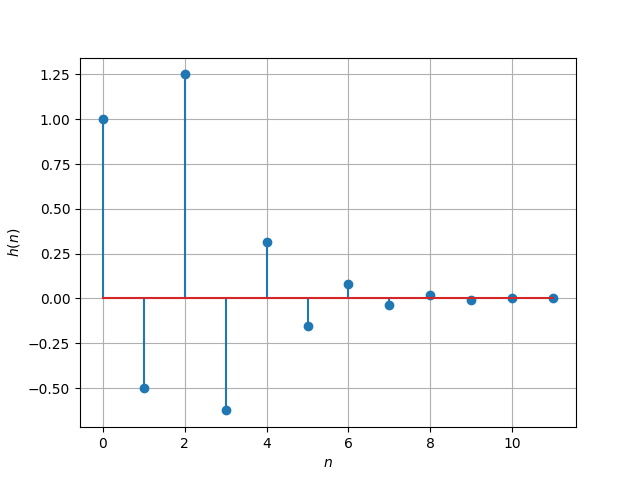
\includegraphics[width=\columnwidth]{figs/5_4.png}
	\caption{$h(n)$ as the inverse of $H(z)$}
	\label{fig:h-n-inv}
\end{figure}
\item Compute 
\begin{equation}
\label{eq:convolution}
y(n) = x(n)*h(n) = \sum_{k=-\infty}^{\infty}x(k)h(n-k)
\end{equation}

Comment. The operation in \eqref{eq:convolution} is known as
{\em convolution}.

\solution The following code plots Fig. \eqref{fig:y-n-conv}. Note that this is the same as $y(n)$ in  Fig. \eqref{fig:xnyn}.
\begin{lstlisting}
$ wget https://raw.githubusercontent.com/Donal-08/EE3900-assignments/main/Assignment_01/codes/5_5.py
\end{lstlisting}
and executed using
\begin{lstlisting}
$ python3 5_5.py
\end{lstlisting}
We use Toeplitz matrices for convolution
\begin{align}
	\mtx{y} &= \mtx{x} \circledast \mtx{h}\\
	\mtx{y} &= 
	\begin{pmatrix}
		h_1 & 0 & . & . & . & 0 \\
		h_2 & h_1 & . & . & . & 0 \\
		h_3 & h_2 & h_1 & . & . & 0 \\
		. & . & . & . & . & . \\
		0 & . & . & h_N & h_{N-1} & h_{N-2} \\
		0 & . & . & . & h_N & h_{N-1} \\
		0 & . & . & . & 0 & h_N
	\end{pmatrix}
	\begin{pmatrix}
		x_1 \\ x_2 \\ \vdots \\ x_n
	\end{pmatrix}
\end{align}
or, equivalently 
\begin{align}
	y[k] = h[n]*x[n] = \sum_{i=-\infty}^{\infty} x[i]h[k-i]
\end{align}

\begin{figure}[!ht]
	\centering
	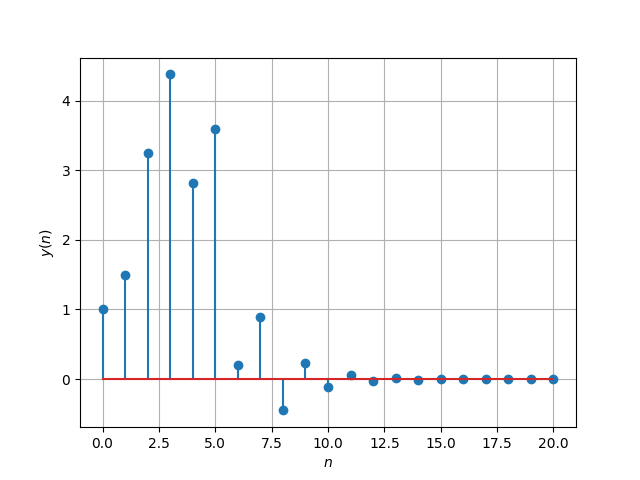
\includegraphics[width=\columnwidth]{figs/5_5.png}
	\caption{$y(n)$ from the definition}
	\label{fig:y-n-conv}
\end{figure}
\item Express the above convolution using a Toeplitz matrix.
	
	\solution Let 
	\begin{align}
		\vec{x} = \myvec{1 \\ 2 \\ 3 \\ 4 \\ 2 \\ 1} \qquad
		\vec{h} = \myvec{1 \\ -0.5 \\ 1.25 \\ -0.62 \\ 0.31 \\ -0.16}
	\end{align}
	
	Their convolution is given by the product of the following Toeplitz matrix $\vec{T}$
	\begin{align}
		&\myvec{
			1 & 0 & 0 & 0 & 0 & 0 \\
			-0.5 & 1 & 0 & 0 & 0 & 0 \\
			1.25 & -0.5 & 1 & 0 & 0 & 0 \\
			-0.62 & 1.25 & -0.5 & 1 & 0 & 0 \\
			0.31 & -0.62 & 1.25 & -0.5 & 1 & 0 \\
			-0.16 & 0.31 & -0.62 & 1.25 & -0.5 & 1 \\
			0 & -0.16 & 0.31 & -0.62 & 1.25 & -0.5 \\
			0 & 0 & -0.16 & 0.31 & -0.62 & 1.25 \\
			0 & 0 & 0 & -0.16 & 0.31 & -0.62 \\
			0 & 0 & 0 & 0 & -0.16 & 0.31 \\
			0 & 0 & 0 & 0 & 0 & -0.16 \\
		} 
	\end{align}
	and $\vec{x}$
	
	\begin{align}
		&\vec{y} = \vec{x} \circledast \vec{h} = \vec{Tx} = \myvec{1 \\ 1.5 \\ 3.25 \\ 4.38 \\ 2.81 \\ 3.59 \\ 0.12 \\ 0.78 \\ -0.62 \\ 0 \\ -0.16}
	\end{align}
	
	Download the following Python code for computing the convolution by using a Toeplitz matrix and plotting Fig. \ref{fig-5.9}
	\begin{lstlisting}
		wget https://github.com/Donal-08/EE3900-assignments/tree/main/Assignment_1/codes/5_9.py
	\end{lstlisting}
	
	Run the Python code by executing
	\begin{lstlisting}
		python 5.9.py
	\end{lstlisting}

	\begin{figure}[!ht]
		\centering
		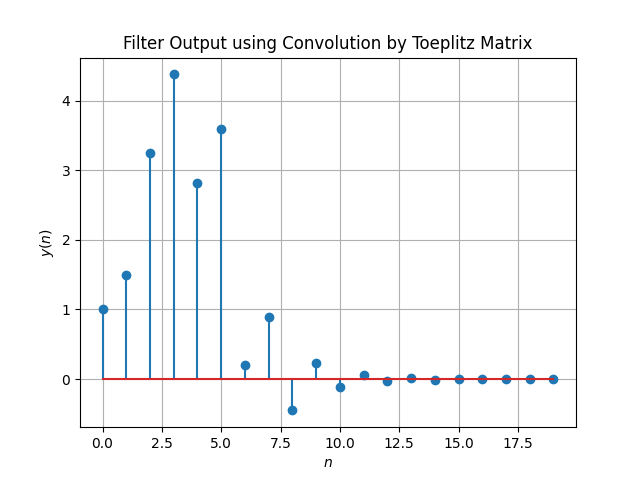
\includegraphics[width=\columnwidth]{figs/5.9.png}
		\caption{Plot of the convolution of $x(n)$ and $h(n)$}
		\label{fig-5.9}	
	\end{figure}
\item Show that
\begin{equation}
y(n) =  \sum_{k=-\infty}^{\infty}x(n-k)h(k)
\end{equation}
\solution 
From \eqref{eq:convolution}, we substitute $k := n - k$ to get
\begin{align}
y\brak{n} &= \sum_{k=-\infty}^{\infty}x\brak{k}h\brak{n - k} \\
		  &= \sum_{n - k=-\infty}^{\infty}x\brak{n - k}h\brak{k} \\
		  &= \sum_{k=-\infty}^{\infty}x\brak{n - k}h\brak{k}
\end{align}
\end{enumerate}

\section{DFT and FFT}
\begin{enumerate}[label=\thesection.\arabic*]
\item
Compute
\begin{equation}
X(k) \define \sum _{n=0}^{N-1}x(n) e^{-\j2\pi kn/N}, \quad k = 0,1,\dots, N-1
\end{equation}
and $H(k)$ using $h(n)$.
\solution The following code plots Fig. \eqref{fig:y-n-dft}. Note that this is the same as $y(n)$ in Fig. \eqref{fig:xnyn}.

\begin{lstlisting}
$ wget https://github.com/Donal-08/EE3900-assignments/blob/main/Assignment_1/codes/6_1.py
\end{lstlisting}
and executed using
\begin{lstlisting}
$ python3 6_1.py
\end{lstlisting}

\begin{figure}[ht!]
	\centering
	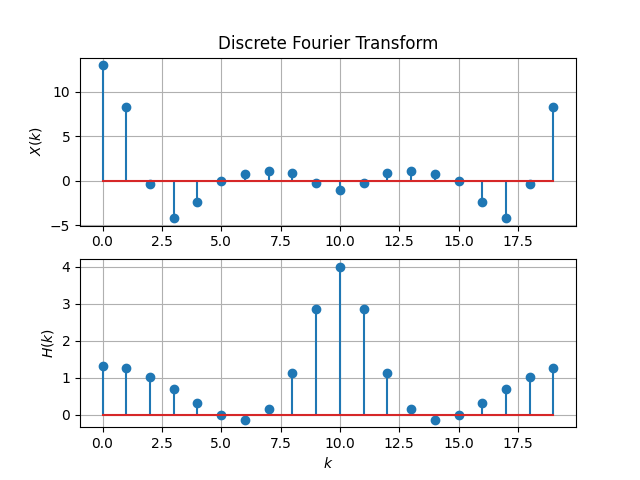
\includegraphics[width=\columnwidth]{figs/6.1.png}
	\caption{DFT of $x(n)$ and $h(n)$}
	\label{fig:y-n-dft}
\end{figure}
\item Compute 
\begin{equation}
Y(k) = X(k)H(k)
\label{eq:fp}
\end{equation}
\solution The following code plots Fig. \eqref{fig:y-n-dft}. Note that this is the same as $y(n)$ in Fig. \eqref{fig:xnyn}.

\begin{lstlisting}
$ wget https://github.com/Donal-08/EE3900-assignments/blob/main/Assignment_1/codes/6_2.py
\end{lstlisting}
and executed using
\begin{lstlisting}
$ python3 6_2.py
\end{lstlisting}
\begin{figure}[!ht]
	\centering
	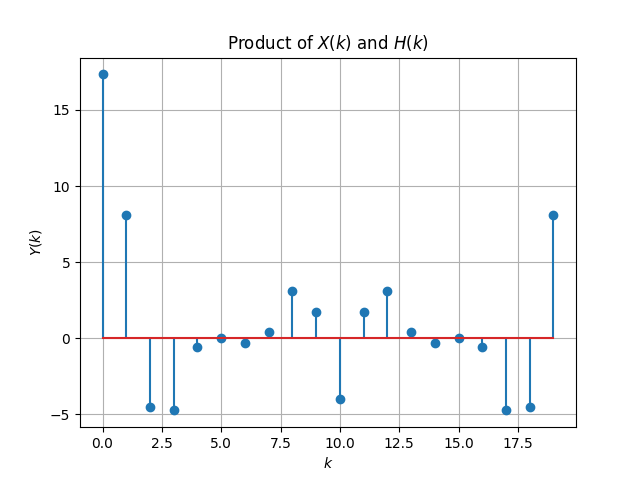
\includegraphics[width=\columnwidth]{figs/6.2.png}
	\caption{$X(k) * H(k)$}
	\label{fig:y-n-dft}
\end{figure}
\item Compute
\begin{equation}
 y\brak{n}={\frac {1}{N}}\sum _{k=0}^{N-1}Y\brak{k}\cdot e^{\j 2\pi kn/N},\quad n = 0,1,\dots, N-1
 \label{eq:inv-ft}
\end{equation}

\solution The following code plots Fig. \eqref{fig:y-n-dft}. Note that this is the same as $y(n)$ in Fig. \eqref{fig:xnyn}.

\begin{lstlisting}
$ wget https://github.com/Donal-08/EE3900-assignments/blob/main/Assignment_1/codes/6_3.py
\end{lstlisting}
and executed using
\begin{lstlisting}
$ python3 6_3.py
\end{lstlisting}

\begin{figure}[!ht]
	\centering
	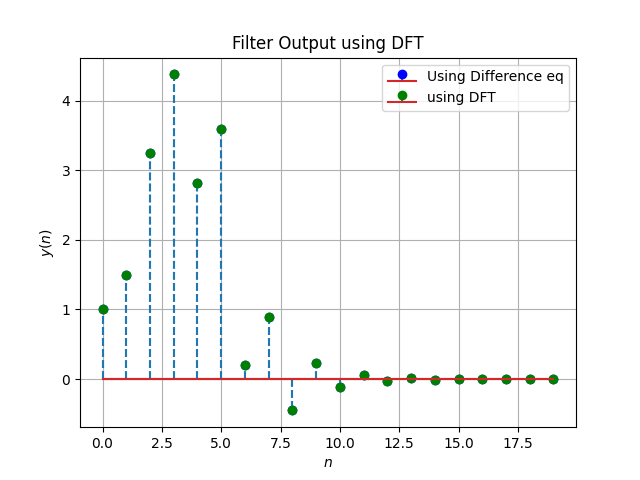
\includegraphics[width=\columnwidth]{figs/6.3.png}
	\caption{$y(n)$ from the IDFT}
	\label{fig:y-n-dft}
\end{figure}
\item Repeat the previous exercise by computing $X(k), H(k)$ and $y(n)$ through FFT and 
% IFFT.

\solution Download the code from
\begin{lstlisting}
$ wget https://github.com/Donal-08/EE3900-assignments/blob/main/Assignment_1/codes/6_4.py
\end{lstlisting}
and execute it using
\begin{lstlisting}
$ python3 6_4.py
\end{lstlisting}
Observe that Fig. \eqref{fig:y-n-fft} is the same as $y(n)$ in Fig. \eqref{fig:xnyn}.

\begin{figure}[h!]
	\centering
	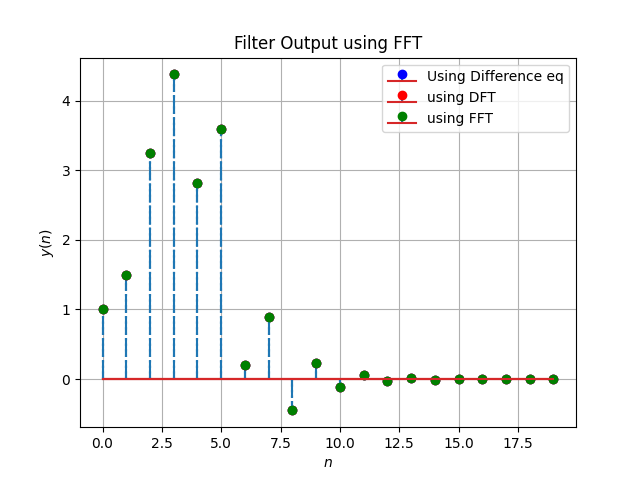
\includegraphics[width=\columnwidth]{figs/6.4.png}
	\caption{$y(n)$ using FFT and IFFT}
	\label{fig:y-n-fft}
\end{figure}
% \item Wherever possible, express all the above equations as matrix equations.

% \solution \begin{align}
% 	\vec{x} &= \myvec{x_0 & x_1	 & \cdots & x_{N-1}}^\top \\
% 	\vec{h} &= \myvec{x_0 & x_1	 & \cdots & x_{N-1}}^\top \\
% 	\vec{y} &= \vec{x} \circledast \vec{h} \\
% 	\myvec{y_1 \\ y_2 \\ \vdots \\ y_{2N - 1}} &= \myvec{
% 		h_0 & 0 & 0 & \cdots & 0 \\
% 		h_1 & h_0 & 0 & \cdots & 0 \\
% 		h_2 & h_1 & h_0 & \cdots & 0 \\
% 		\vdots & \vdots & \vdots & \ddots & \vdots \\
% 		h_{N-1} & h_{N-2} & h_{N-3} & \cdots & h_0 \\
% 		0 & h_{N-1} & h_{N-2} & \cdots & h_1 \\
% 		0 & 0 & h_{N-1} & \cdots & h_2 \\
% 		\vdots & \vdots & \vdots & \ddots & \vdots \\
% 		0 & 0 & 0 & \cdots & h_{N-1}
% 	}		
% 	\myvec{x_1\\x_2\\ \vdots \\x_N}
% \end{align}
% We use the DFT Matrix, where $\omega_n = e^{-\frac{j2k\pi}{n}}$, which is given by
% \begin{align}
% 	\mtx{W} = 
% 	\begin{pmatrix}
% 		1 & 1 & \ldots & 1 \\
% 		1 & \omega_n^1 & \ldots & \omega_n^{n - 1} \\
% 		\vdots & \vdots & \ddots & \vdots \\
% 		1 & \omega_n^{n - 1} & \ldots & \omega_n^{(n -1)(n - 1)}
% 	\end{pmatrix}
% \end{align}
% i.e. $W_{jk} = \omega^{jk}$, $0 \leq j, k < n$. Hence, we can write any DFT equation as
% \begin{align}
% 	\mtx{X} = \mtx{W}\mtx{x} = \mtx{x}\mtx{W}
% \end{align}
% \noindent where
% \begin{align}
% 	\mtx{x} = 
% 	\begin{pmatrix}
% 		x(0) \\ x(1) \\ \vdots \\ x(n - 1)
% 	\end{pmatrix}
% \end{align}
% \noindent Using \eqref{eq:inv-ft}, the inverse Fourier Transform is given by
% \begin{align}
% 	\mtx{x} = \mathcal{F}^{-1}\brak{\mtx{X}} = \mtx{W}^{-1}\mtx{X} &= \frac{1}{N}\mtx{W^{H}}\mtx{X} = \frac{1}{N}\mtx{X}\mtx{W^{H}} \\ 
% 	\implies \mtx{W}^{-1} &= \frac{1}{N}\mtx{W^{H}}
% \end{align}
% \noindent where $H$ denotes hermitian operator. We can rewrite \eqref{eq:fp} using the element-wise multiplication operator as
% \begin{align}
% 	\mtx{Y} = \mtx{H}\cdot\mtx{X} = \brak{\mtx{W}\mtx{h}}\cdot\brak{\mtx{W}\mtx{x}}
% \end{align}
% \item Verify the above equation by generating the DFT matrix in python.\\
% \solution Download the code from
% \begin{lstlisting}
% wget https://github.com/Donal-08/EE3900/blob/main/Assignment_1/codes/6.6.py
% \end{lstlisting}
% and execute it using
% \begin{lstlisting}
% $ python3 6.6.py
% \end{lstlisting}
% \begin{figure}[ht!]
% 	\centering
% 	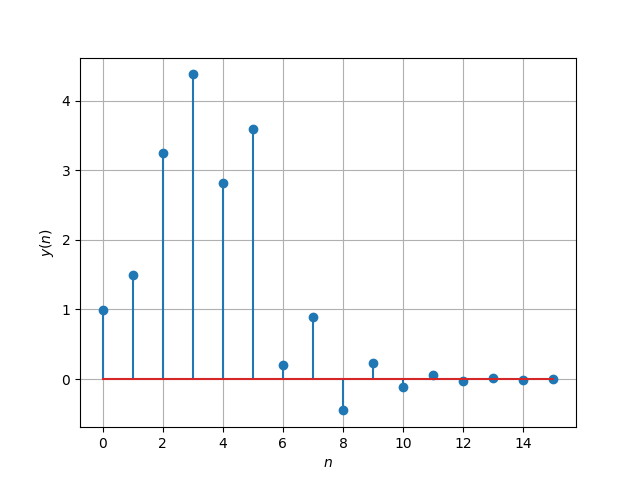
\includegraphics[width=\columnwidth]{figs/6.6.png}
% 	\caption{$y(n)$ using FFT and IFFT}
% 	\label{}
% \end{figure}
\end{enumerate}

\section{FFT}
\begin{enumerate}[label=\thesection.\arabic*]
\item The DFT of $x(n)$ is given by
\begin{align}
	X(k) \triangleq \sum_{n=0}^{N-1} x(n) e^{-j 2 \pi k n / N}, \quad k=0,1, \ldots, N-1
\end{align}

\item Let 
\begin{align}
	W_{N} = e^{-j2\pi/N} 
\end{align}
	Then the $N$-point {\em DFT matrix} is defined as 
\begin{align}
	\vec{F}_{N} = \sbrak{W_{N}^{mn}}, \quad 0 \le m,n \le N-1 
\end{align}
where $W_{N}^{mn}$ are the elements of $\vec{F}_{N}$.

\item Let 
\begin{align}
	\vec{I}_4 = \myvec{\vec{e}_4^{1} &\vec{e}_4^{2} &\vec{e}_4^{3} &\vec{e}_4^{4} }
\end{align}
	be the $4\times 4$ identity matrix.  Then the 4 point {\em DFT permutation matrix} is defined as 
\begin{align}
	\vec{P}_4 = \myvec{\vec{e}_4^{1} &\vec{e}_4^{3} &\vec{e}_4^{2} &\vec{e}_4^{4} }
\end{align}

\item The 4 point {\em DFT diagonal matrix} is defined as 
\begin{align}
	\vec{D}_4 = \mathrm{diag}\myvec{W_{8}^{0} & W_{8}^{1} & W_{8}^{2} & W_{8}^{3}}
\end{align}

\item Show that 
\begin{equation}
		W_{N}^{2}=W_{N/2}
\end{equation}

\solution
\begin{align}
	W_N^2 &= \brak{\exp\brak{-j\frac{2\pi}{N}}}^2	 \\
	&= \exp\brak{-j\frac{2\pi}{N} \cdot 2} \\
	&= \exp\brak{-j\frac{2\pi}{N/2}} \\
	&= W_{N/2}
\end{align}	 

%    \item Find $\vec{P}_6$.
%    \item Find $\vec{D}_3$.
\item Show that 
\begin{equation}
\vec{F}_{4}=
\begin{bmatrix}
\vec{I}_{2} & \vec{D}_{2} \\
\vec{I}_{2} & -\vec{D}_{2}
\end{bmatrix}
\begin{bmatrix}
\vec{F}_{2} & 0 \\
0 & \vec{F}_{2}
\end{bmatrix}
\vec{P}_{4}
\end{equation}

\solution
\begin{align}
	&\mymat{\vec{I}_2 & \vec{D}_2 \\ \vec{I}_2 & -\vec{D}_2} \mymat{\vec{F}_2 & 0 \\ 0 & \vec{F}_2} \\
	= &\mymat{\vec{F}_2 & \vec{D}_2\vec{F}_2 \\ \vec{F}_2 & -\vec{D}_2\vec{F}_2}  \\
	= &\mymat{\myvec{1&1\\1&-1} & \myvec{1&0\\0&-\j}\myvec{1&1\\1&-1} \\ \myvec{1&1\\1&-1} & - \myvec{1&0\\0&-\j}\myvec{1&1\\1&-1}} \\
	= &\mymat{1 & 1 & 1 & 1 \\ 1 & -1 & -\j & \j \\ 1 & 1 & -1 & -1 \\ 1 & -1 & \j & -\j}
\end{align}		
because $W_2^0 = 1$ and $W_2^1 = e^{-\j\pi} = -1$

Now
\begin{align}
	&\mymat{\vec{I}_2 & \vec{D}_2 \\ \vec{I}_2 & -\vec{D}_2} \mymat{\vec{F}_2 & 0 \\ 0 & \vec{F}_2} \vec{P}_4 \\
	= &\mymat{1 & 1 & 1 & 1 \\ 1 & -1 & -\j & \j \\ 1 & 1 & -1 & -1 \\ 1 & -1 & \j & -\j} \mymat{1 & 0 & 0 & 0 \\ 0 & 0 & 1 & 0 \\ 0 & 1 & 0 & 0 \\ 0 & 0 & 0 & 1} \\
	= &\mymat{1 & 1 & 1 & 1 \\ 1 & -\j & -1 & \j \\ 1 & -1 & 1 & -1 \\ 1 & \j & -1 & -\j} \\
	= &\mymat{W_4^0 & W_4^0 & W_4^0 & W_4^0 \\ W_4^0 & W_4^1 & W_4^2 & W_4^3 \\ W_4^0 & W_4^2 & W_4^4 & W_4^6 \\ W_4^0 & W_4^3 & W_4^6 & W_4^9} \\
	= &~\vec{F}_4
\end{align}
because
\begin{align}
	W_4^0 &= 1 \\
	W_4^1 &= e^{-\j\frac{\pi}{2}} = -\j \\
	W_4^2 &= e^{-\j\pi} = -1 \\
	W_4^3 &= e^{-\j\frac{3\pi}{2}} = \j \\
	W_4^n &= W_4^{n - 4} &&\forall n \ge 4
\end{align}	 	

\item Show that 
\begin{equation}
\vec{F}_{N}=
\begin{bmatrix}
\vec{I}_{N/2} & \vec{D}_{N/2} \\
\vec{I}_{N/2} & -\vec{D}_{N/2}
\end{bmatrix}
\begin{bmatrix}
\vec{F}_{N/2} & 0 \\
0 & \vec{F}_{N/2}
\end{bmatrix}
\vec{P}_{N}
\end{equation}

\solution
\begin{align}
	&\mymat{\vec{I}_{N/2} & \vec{D}_{N/2} \\ \vec{I}_{N/2} & -\vec{D}_{N/2}} \mymat{\vec{F}_{N/2} & 0 \\ 0 & \vec{F}_{N/2}}  \\
	= &\mymat{\vec{F}_{N/2} & \vec{D}_{N/2}\vec{F}_{N/2} \\ \vec{F}_{N/2} & -\vec{D}_{N/2}\vec{F}_{N/2}}
\end{align}

Now
\begin{align}
	&\vec{D}_{N/2}\vec{F}_{N/2} \\
	&= \mymat{W_N^0 & \cdots & 0 \\ \vdots & \ddots & \vdots \\ 0 & \cdots & W_N^{N/2-1}} \mymat{W_{N/2}^0 & \cdots & W_{N/2}^0 \\ \vdots & \ddots & \vdots \\ W_{N/2}^0 & \cdots & W_{N/2}^{(N/2 - 1)^2}} \\
	&= \mymat{W_N^0 W_{N/2}^0 & \cdots & W_N^0 W_{N/2}^0 \\ \vdots & \ddots & \vdots \\ W_N^{N/2-1} W_{N/2}^0 & \cdots & W_N^{N/2-1} W_{N/2}^{(N/2 - 1)^2}} 
\end{align}

Thus
\begin{align}
	\brak{\vec{D}_{N/2}\vec{F}_{N/2}}_{ij} &= W_N^i W_{N/2}^{ij} \\
	&= W_N^i W_N^{2ij} \\
	&= W_N^{i(2j + 1)}
\end{align}
where $i, j = 0, \ldots, N/2 - 1$

Therefore, $\vec{D}_{N/2}\vec{F}_{N/2}$ forms the first $N/2$ rows of the odd-indexed columns of $\vec{F}_N$
\begin{align}
	W_N^{(i + N/2)(2j + 1)} &= \exp\brak{-\j \frac{2\pi}{N} (2j + 1)\brak{i + \frac{N}{2}}} \\
	&= \exp\brak{-\j \brak{\frac{2\pi}{N} (2j + 1)i + (2j + 1)\pi}} \\
	&= -\exp\brak{-\j \frac{2\pi}{N} (2j + 1)i} \\
	&= -W_N^{i(2j + 1)}
\end{align}

Thus, the remaining $N/2$ rows will be the negatives of the first $N/2$ rows
\begin{align}
	\brak{\vec{F}_{N/2}}_{ij} &= W_{N/2}^{ij} \\
	&= W_N^{i(2j)}
\end{align}
where $i, j = 0, \ldots, N/2 - 1$

Therefore, $\vec{F}_{N/2}$ forms the first $N/2$ rows of the even-indexed columns of $\vec{F}_N$
\begin{align}
	W_N^{(i + N/2)(2j)} &= \exp\brak{-\j \frac{2\pi}{N} (2j)\brak{i + \frac{N}{2}}} \\
	&= \exp\brak{-\j \brak{\frac{2\pi}{N} (2j)i + (2j)\pi}} \\
	&= \exp\brak{-\j \frac{2\pi}{N} (2j)i} \\
	&= W_N^{i(2j)}
\end{align}
Thus, the remaining $N/2$ rows will be the same as the first $N/2$ rows

Therefore
\begin{align}
	\mymat{\vec{F}_{N/2} & \vec{D}_{N/2}\vec{F}_{N/2} \\ \vec{F}_{N/2} & -\vec{D}_{N/2}\vec{F}_{N/2}} = \vec{F}_N \vec{P}_N
\end{align}
where 
\begin{align}
	\vec{P}_N = \myvec{\vec{e}_N^1 & \vec{e}_N^3 & \cdots & \vec{e}_N^{N-1} & \vec{e}_N^2 & \vec{e}_N^4 & \cdots & \vec{e}_N^N}
\end{align}

Hence
\begin{align}
	\mymat{\vec{F}_{N/2} & \vec{D}_{N/2}\vec{F}_{N/2} \\ \vec{F}_{N/2} & -\vec{D}_{N/2}\vec{F}_{N/2}} \vec{P}_N = \vec{F}_N \vec{P}_N^2 = \vec{F}_N \\
	\therefore \vec{F}_N = \mymat{\vec{I}_{N/2} & \vec{D}_{N/2} \\ \vec{I}_{N/2} & -\vec{D}_{N/2}} \mymat{\vec{F}_{N/2} & 0 \\ 0 & \vec{F}_{N/2}} \vec{P}_N
\end{align}
for even $N$

\item Find 
\begin{align}
	 \vec{P}_4 \vec{x}
\end{align}

\solution Let $\vec{x} = \myvec{x(0) & x(1) & x(2) & x(3)}^\top$
\begin{align}
	\vec{P}_4 \vec{x} &= \mymat{1 & 0 & 0 & 0 \\ 0 & 0 & 1 & 0 \\ 0 & 1 & 0 & 0 \\ 0 & 0 & 0 & 1} \mymat{x(0) \\ x(1) \\ x(2) \\ x(3)} \\
	&= \mymat{x(0) \\ x(2) \\ x(1) \\ x(3)}
\end{align}

\item Show that 
\begin{align}
	\vec{X} = \vec{F}_N \vec{x}
	\label{eq:dft-mat-def}
\end{align}
	where $\vec{x}, \vec{X}$ are the vector representations of $x(n), X(k)$ respectively.
	
\solution
\begin{align}
	X(k) &= \sum_{n=0}^{N-1} x(n) e^{-j 2 \pi k n / N}, \quad k=0,1, \ldots, N-1 \\
	\implies \vec{X} &= \mymat{\sum_{n=0}^{N-1} x(n) e^{-j 2 \pi  n (0) / N} \\ \vdots \\ \sum_{n=0}^{N-1} x(n) e^{-j 2 \pi  n (N-1) / N}} \\
	&= \mymat{x(0) + \cdots + x(N-1) \\ \vdots \\ x(0) + \cdots + x(N-1) e^{-j 2 \pi (N-1)^2 / N}} 
\end{align}
\begin{align}
		\vec{X} &= x(0) \mymat{1 \\ \vdots \\ 1} + \cdots + x(N-1)\mymat{1 \\ \vdots \\ e^{-j 2 \pi (N-1)^2 / N}} \\
		&= \mymat{1 & \cdots & 1 \\ \vdots & \ddots & \vdots \\ 1 & \cdots & e^{-j 2 \pi (N-1)^2 / N}} \mymat{x(0) \\ \vdots \\ x(N-1)} \\
		&= \vec{F}_N \vec{x}
\end{align}
	
\item Derive the following step-by-step visualisation  of
8-point FFTs into 4-point FFTs and so on
\begin{equation}
\begin{bmatrix}
X(0) \\ 
X(1) \\ 
X(2) \\ 
X(3)
\end{bmatrix}
=
\begin{bmatrix}
X_{1}(0) \\ 
X_{1}(1)\\ 
X_{1}(2)\\
X_{1}(3)\\
\end{bmatrix}
+
\begin{bmatrix}
W^{0}_{8} & 0 & 0 & 0\\
0 & W^{1}_{8} & 0 & 0\\
0 & 0 & W^{2}_{8} & 0\\
0 & 0 & 0 & W^{3}_{8}
\end{bmatrix}
\begin{bmatrix}
X_{2}(0) \\ 
X_{2}(1) \\ 
X_{2}(2) \\
X_{2}(3)
\end{bmatrix}
\end{equation}
\begin{equation}
\begin{bmatrix}
X(4) \\ 
X(5) \\ 
X(6) \\ 
X(7)
\end{bmatrix}
=
\begin{bmatrix}
X_{1}(0) \\ 
X_{1}(1)\\ 
X_{1}(2)\\
X_{1}(3)\\
\end{bmatrix}
-
\begin{bmatrix}
W^{0}_{8} & 0 & 0 & 0\\
0 & W^{1}_{8} & 0 & 0\\
0 & 0 & W^{2}_{8} & 0\\
0 & 0 & 0 & W^{3}_{8}
\end{bmatrix}
\begin{bmatrix}
X_{2}(0) \\ 
X_{2}(1) \\ 
X_{2}(2) \\
X_{2}(3)
\end{bmatrix}
\end{equation}
4-point FFTs into 2-point FFTs
\begin{equation}
\begin{bmatrix}
X_{1}(0) \\ 
X_{1}(1)\\ 
\end{bmatrix}
=
\begin{bmatrix}
X_{3}(0) \\ 
X_{3}(1)\\ 
\end{bmatrix}
+
\begin{bmatrix}
W^{0}_{4} & 0\\
0 & W^{1}_{4}
\end{bmatrix}
\begin{bmatrix}
X_{4}(0) \\ 
X_{4}(1) \\ 
\end{bmatrix}
\end{equation}
\begin{equation}
\begin{bmatrix}
X_{1}(2) \\ 
X_{1}(3)\\ 
\end{bmatrix}
=
\begin{bmatrix}
X_{3}(0) \\ 
X_{3}(1)\\ 
\end{bmatrix}
-
\begin{bmatrix}
W^{0}_{4} & 0\\
0 & W^{1}_{4}
\end{bmatrix}
\begin{bmatrix}
X_{4}(0) \\ 
X_{4}(1) \\ 
\end{bmatrix}
\end{equation}
\begin{equation}
\begin{bmatrix}
X_{2}(0) \\ 
X_{2}(1)\\ 
\end{bmatrix}
=
\begin{bmatrix}
X_{5}(0) \\ 
X_{5}(1)\\ 
\end{bmatrix}
+
\begin{bmatrix}
W^{0}_{4} & 0\\
0 & W^{1}_{4}
\end{bmatrix}
\begin{bmatrix}
X_{6}(0) \\ 
X_{6}(1) \\ 
\end{bmatrix}
\end{equation}
\begin{equation}
\begin{bmatrix}
X_{2}(2) \\ 
X_{2}(3)\\ 
\end{bmatrix}
=
\begin{bmatrix}
X_{5}(0) \\ 
X_{5}(1)\\ 
\end{bmatrix}
-
\begin{bmatrix}
W^{0}_{4} & 0\\
0 & W^{1}_{4}
\end{bmatrix}
\begin{bmatrix}
X_{6}(0) \\ 
X_{6}(1) \\ 
\end{bmatrix}
\end{equation}
\begin{equation}
\vec{P}_{8}
\begin{bmatrix}
x(0) \\ 
x(1) \\ 
x(2) \\ 
x(3) \\ 
x(4) \\ 
x(5) \\
x(6) \\
x(7)
\end{bmatrix}
= 
\begin{bmatrix}
x(0) \\ 
x(2) \\ 
x(4) \\ 
x(6) \\
x(1) \\ 
x(3) \\ 
x(5) \\
x(7)
\end{bmatrix}
\end{equation}
\begin{equation}
\vec{P}_{4}
\begin{bmatrix}
x(0) \\ 
x(2) \\ 
x(4) \\ 
x(6) \\
\end{bmatrix}
= 
\begin{bmatrix}
x(0) \\ 
x(4) \\ 
x(2) \\
x(6)
\end{bmatrix}
\end{equation}
\begin{equation}
\vec{P}_{4}
\begin{bmatrix}
x(1) \\ 
x(3) \\ 
x(5) \\
x(7)
\end{bmatrix}
= 
\begin{bmatrix}
x(1) \\ 
x(5) \\ 
x(3) \\ 
x(7) \\
\end{bmatrix}
\end{equation}
Therefore,
\begin{equation}
\begin{bmatrix}
X_{3}(0) \\ 
X_{3}(1)\\ 
\end{bmatrix}
= \vec{F}_{2}
\begin{bmatrix}
x(0) \\ 
x(4) \\ 
\end{bmatrix}
\end{equation}
\begin{equation}
\begin{bmatrix}
X_{4}(0) \\ 
X_{4}(1)\\ 
\end{bmatrix}
= \vec{F}_{2}
\begin{bmatrix}
x(2) \\ 
x(6) \\ 
\end{bmatrix}
\end{equation}
\begin{equation}
\begin{bmatrix}
X_{5}(0) \\ 
X_{5}(1)\\ 
\end{bmatrix}
= \vec{F}_{2}
\begin{bmatrix}
x(1) \\ 
x(5) \\ 
\end{bmatrix}
\end{equation}
\begin{equation}
\begin{bmatrix}
X_{6}(0) \\ 
X_{6}(1)\\ 
\end{bmatrix}
= \vec{F}_{2}
\begin{bmatrix}
x(3) \\ 
x(7) \\ 
\end{bmatrix}
\end{equation}

\solution 
\begin{align}
	X(k) &= \sum_{n=0}^7 x(n) e^{-j 2 \pi k n / 8}, \quad k=0, \ldots, 7\\
	&= \sum_{n=0}^7 x(n) W_8^{kn} \\
	&= \sum_{n \text{ is even}}x(n) W_8^{kn} + \sum_{n \text{ is odd}}x(n) W_8^{kn} \\
	&= \sum_{m=0}^3 x(2m) W_8^{2km} + \sum_{m=0}^3 x(2m+1) W_8^{2km + k}
\end{align}	

Now substitute $W_8^2 = W_4$
\begin{align}
		X(k) = \sum_{m=0}^3 x(2m) W_4^{km} + W_8^k \sum_{m=0}^3 x(2m+1) W_4^{km}
\end{align}

Consider
\begin{align}
		x_1(n) = \cbrak{x(0), x(2), x(4), x(6)} \\
		x_2(n) = \cbrak{x(1), x(3), x(5), x(7)}
\end{align}

Thus
\begin{align}
		X(k) = X_1(k) + W_8^k X_2(k) \qquad k = 0,\ldots,7
\end{align}

Now, $X_1(k)$ and $X_2(k)$ are $4$-point DFTs which means they are periodic with period $4$
\begin{align}
		X(k+4) &= X_1(k+4) + W_8^{k+4} X_2(k+4) \\
		&= X_1(k) + e^{-\j 2\pi(k+4)/8} X_2(k) \\
		&= X_1(k) + e^{-\j (2\pi k/8 + \pi)} X_2(k) \\
		&= X_1(k) - e^{-\j 2\pi k/8 } X_2(k) \\
		&= X_1(k) - W_8^k X_2(k)
\end{align}

Therefore, for $k=0,1,2,3$
\begin{align}
		X(k) = X_1(k) + W_8^k X_2(k)  \\
		X(k+4) = X_1(k) - W_8^k X_2(k) 
\end{align}

which is the same as
\begin{equation}
\begin{bmatrix}
X(0) \\ 
X(1) \\ 
X(2) \\ 
X(3)
\end{bmatrix}
=
\begin{bmatrix}
X_{1}(0) \\ 
X_{1}(1)\\ 
X_{1}(2)\\
X_{1}(3)\\
\end{bmatrix}
+
\begin{bmatrix}
W^{0}_{8} & 0 & 0 & 0\\
0 & W^{1}_{8} & 0 & 0\\
0 & 0 & W^{2}_{8} & 0\\
0 & 0 & 0 & W^{3}_{8}
\end{bmatrix}
\begin{bmatrix}
X_{2}(0) \\ 
X_{2}(1) \\ 
X_{2}(2) \\
X_{2}(3)
\end{bmatrix}
\end{equation}
\begin{equation}
\begin{bmatrix}
X(4) \\ 
X(5) \\ 
X(6) \\ 
X(7)
\end{bmatrix}
=
\begin{bmatrix}
X_{1}(0) \\ 
X_{1}(1)\\ 
X_{1}(2)\\
X_{1}(3)\\
\end{bmatrix}
-
\begin{bmatrix}
W^{0}_{8} & 0 & 0 & 0\\
0 & W^{1}_{8} & 0 & 0\\
0 & 0 & W^{2}_{8} & 0\\
0 & 0 & 0 & W^{3}_{8}
\end{bmatrix}
\begin{bmatrix}
X_{2}(0) \\ 
X_{2}(1) \\ 
X_{2}(2) \\
X_{2}(3)
\end{bmatrix}
\end{equation}

Similarly, we can divide $x_1(n)$ into 
\begin{align}
	x_3(n) = \cbrak{x(0), x(4)} \\
	x_4(n) = \cbrak{x(2), x(6)}
\end{align}
i.e.,
\begin{align}
	\mymat{X_3(0) \\ X_3(1)} = \vec{F}_2 \mymat{x(0) \\ x(4)} \\
	\mymat{X_4(0) \\ X_4(1)} = \vec{F}_2 \mymat{x(2) \\ x(6)}
\end{align}
to get
\begin{align}
	X_1(k) = X_3(k) + W_4^k X_4(k) \\
	X_1(k + 2) = X_3(k) - W_4^k X_4(k) 
\end{align}
for $k = 0, 1$
\begin{equation}
\begin{bmatrix}
X_{1}(0) \\ 
X_{1}(1)\\ 
\end{bmatrix}
=
\begin{bmatrix}
X_{3}(0) \\ 
X_{3}(1)\\ 
\end{bmatrix}
+
\begin{bmatrix}
W^{0}_{4} & 0\\
0 & W^{1}_{4}
\end{bmatrix}
\begin{bmatrix}
X_{4}(0) \\ 
X_{4}(1) \\ 
\end{bmatrix}
\end{equation}
\begin{equation}
\begin{bmatrix}
X_{1}(2) \\ 
X_{1}(3)\\ 
\end{bmatrix}
=
\begin{bmatrix}
X_{3}(0) \\ 
X_{3}(1)\\ 
\end{bmatrix}
-
\begin{bmatrix}
W^{0}_{4} & 0\\
0 & W^{1}_{4}
\end{bmatrix}
\begin{bmatrix}
X_{4}(0) \\ 
X_{4}(1) \\ 
\end{bmatrix}
\end{equation}

And on dividing $x_2(n)$ into
\begin{align}
	x_5(n) = \cbrak{x(1), x(5)} \\
	x_6(n) = \cbrak{x(3), x(7)}
\end{align}
i.e.,
\begin{align}
	\mymat{X_5(0) \\ X_5(1)} = \vec{F}_2 \mymat{x(1) \\ x(5)} \\
	\mymat{X_6(0) \\ X_6(1)} = \vec{F}_2 \mymat{x(3) \\ x(7)}
\end{align}
to get
\begin{align}
	X_2(k) = X_5(k) + W_4^k X_6(k) \\
	X_2(k + 2) = X_5(k) - W_4^k X_6(k) 
\end{align}
for $k = 0, 1$
\begin{equation}
\begin{bmatrix}
X_{2}(0) \\ 
X_{2}(1)\\ 
\end{bmatrix}
=
\begin{bmatrix}
X_{5}(0) \\ 
X_{5}(1)\\ 
\end{bmatrix}
+
\begin{bmatrix}
W^{0}_{4} & 0\\
0 & W^{1}_{4}
\end{bmatrix}
\begin{bmatrix}
X_{6}(0) \\ 
X_{6}(1) \\ 
\end{bmatrix}
\end{equation}
\begin{equation}
\begin{bmatrix}
X_{2}(2) \\ 
X_{2}(3)\\ 
\end{bmatrix}
=
\begin{bmatrix}
X_{5}(0) \\ 
X_{5}(1)\\ 
\end{bmatrix}
-
\begin{bmatrix}
W^{0}_{4} & 0\\
0 & W^{1}_{4}
\end{bmatrix}
\begin{bmatrix}
X_{6}(0) \\ 
X_{6}(1) \\ 
\end{bmatrix}
\end{equation}

\item For 
\begin{align}
	\vec{x} = \myvec{1\\2\\3\\4\\2\\1}
	\label{eq:equation1}
\end{align}
compute the DFT  
	using 
	\eqref{eq:dft-mat-def}
	
\solution Download the following Python code that plots Fig. \ref{fig-7.11}.
\begin{lstlisting}
	wget https://github.com/Donal-08/EE3900/raw/main/Assignment_1/codes/7.11.py
\end{lstlisting}

Run the code by executing
\begin{lstlisting}
	python 7.11.py
\end{lstlisting} 
\begin{figure}[!ht]
	\centering
	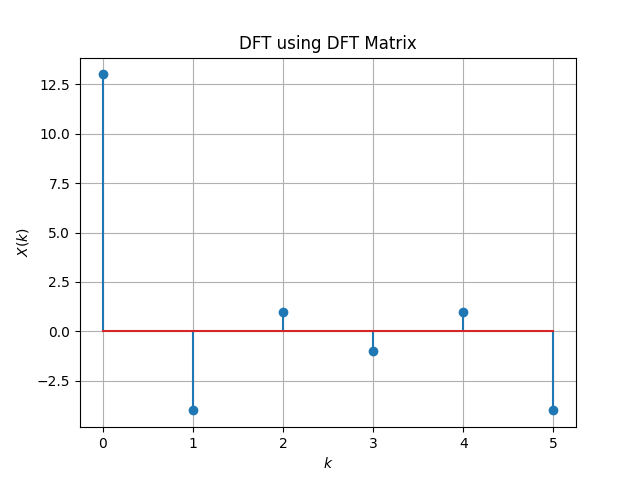
\includegraphics[width=\columnwidth]{figs/7.11.png}
	\caption{Plot of DFT of $\vec{x}$}
	\label{fig-7.11}	
\end{figure}
\item Repeat the above exercise using the FFT
				after zero padding $\vec{x}$. \\
		%	    \eqref{eq:fft-mat-def}
		\solution Download the following Python code that plots Fig. \ref{fig-7.12}.
		\begin{lstlisting}
			wget https://github.com/Donal-08/EE3900/raw/main/Assignment_1/codes/7.12.py
		\end{lstlisting}
		
		Run the code by executing
		\begin{lstlisting}
			python 7.12.py
		\end{lstlisting}
	
		\begin{figure}[!ht]
			\centering
			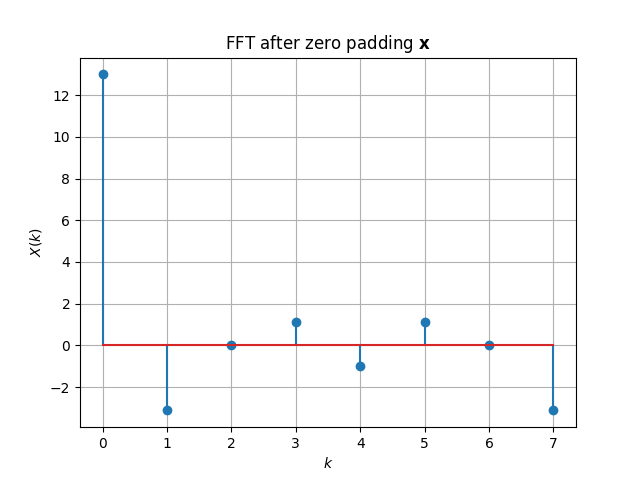
\includegraphics[width=\columnwidth]{./figs/7.12.png}
			\caption{Plot of the fast fourier transform of $\vec{x}$ after zero padding}
			\label{fig-7.12}	
		\end{figure}
		\item Write a C program to compute the 8-point FFT.\\
		\solution Download the following C codes that generate the values of $X(k)$ using $8$-point FFT
		\begin{lstlisting}
			wget https://github.com/Donal-08/EE3900/raw/main/Assignment_1/codes/header.h
			wget https://github.com/Donal-08/EE3900/raw/main/Assignment_1/codes/7.13.c
		\end{lstlisting}
		
		Compile and run the C program by executing the following
		\begin{lstlisting}
			cc -lm 7.13.c
			./a.out
		\end{lstlisting}
		
		Download the following Python code that plots Fig. \ref{fig-7.13} using the data generated by the above C code
		\begin{lstlisting}
			wget https://github.com/Donal-08/EE3900/raw/main/Assignment_1/codes/7.13.py
		\end{lstlisting}
		
		Run the code by executing
		\begin{lstlisting}
			python 7.13.py
		\end{lstlisting}
	
		\begin{figure}[!ht]
			\centering
			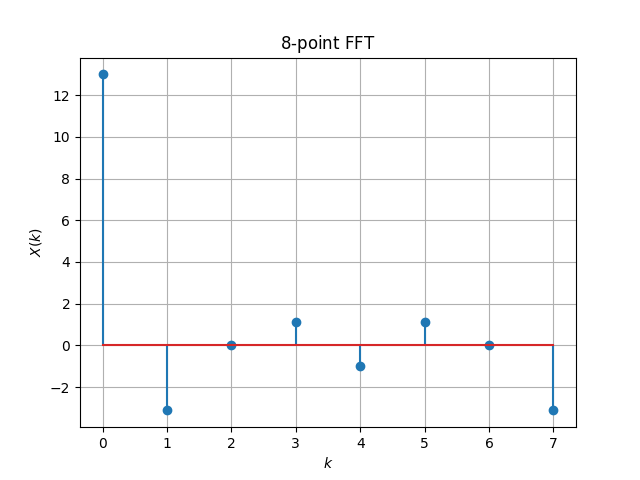
\includegraphics[width=\columnwidth]{figs/7.13.png}
			\caption{Plot of $\vec{X}$ by $8$-point FFT}
			\label{fig-7.13}	
		\end{figure} 
\end{enumerate}


\section{Exercises}
	Answer the following questions by looking at the python code in Problem \ref{prob:output}
	
	\begin{enumerate}[label=\thesection.\arabic*]
	\item The command
	\begin{lstlisting}
		output_signal = signal.lfilter(b, a, input_signal)
	\end{lstlisting}
	in Problem \ref{prob:output} is executed through the following difference equation
	\begin{equation}
		\label{eq:iir_filter_gen}
 		\sum _{m=0}^{M}a\brak{m}y\brak{n-m}=\sum _{k=0}^{N}b\brak{k}x\brak{n-k}
	\end{equation}
	where the input signal is $x(n)$ and the output signal is $y(n)$ with initial values all 0. Replace \textbf{signal.filtfilt} with your own routine and verify.
	
	\solution On taking the $Z$-transform on both sides of the difference equation
	\begin{align}
		\sum _{m=0}^{M}a\brak{m} z^{-m} Y(z) &= \sum _{k=0}^{N}b\brak{k} z^{-k} X(z) \\
		\implies H(z) = \frac{Y(z)}{X(z)} &= \frac{\sum _{k=0}^{N}b\brak{k} z^{-k}}{\sum _{m=0}^{M}a\brak{m} z^{-m}}
	\end{align}
	
	For obtaining the discrete Fourier transform, put $z = \j \frac{2\pi i}{I}$ where $I$ is the length of the input signal and $i = 0, 1, \ldots, I-1$
	
	Download the following Python code that does the above
	\begin{lstlisting}
		wget https://github.com/Donal-08/EE3900/raw/main/Assignment_1/codes/7.1.py
	\end{lstlisting}
	
	Run the code by executing
	\begin{lstlisting}
		python 7.1.py
	\end{lstlisting}
	
	\item Repeat all the exercises in the previous sections for the above $a$ and $b$
	
	\solution The polynomial coefficients obtained are
	\begin{align}
		\vec{a} = \myvec{1.000 \\ -2.519 \\ 2.561 \\ -1.206 \\ 0.220} \qquad
		\vec{b} = \myvec{0.003 \\ 0.014 \\ 0.021 \\ 0.014 \\ 0.003}
	\end{align}
	
	The difference equation is then given by
	\begin{equation}
		\vec{a}^\top \vec{y} = \vec{b}^\top \vec{x} 
	\end{equation}
	
	where
	\begin{align}
		\vec{y} = \myvec{y(n) \\ y(n-1) \\ y(n-2) \\ y(n-3) \\ y(n-4)} \qquad
		\vec{x} = \myvec{x(n) \\ x(n-1) \\ x(n-2) \\ x(n-3) \\ x(n-4)}
	\end{align}
	
	We have
	\begin{equation}
		H(z) = \frac{Y(z)}{X(z)} = \frac{\sum _{k=0}^{N}b\brak{k} z^{-k}}{\sum _{m=0}^{M}a\brak{m} z^{-m}}
	\end{equation}
	
	By using partial fraction decomposition, we can write this as
	\begin{equation}
		H(z) = \sum_i \frac{r(i)}{1-p(i)z^{-1}} + \sum_j k(j)z^{-j}
	\end{equation}
	
	On taking the inverse $Z$-transform on both sides by using \eqref{eq:anun}
	\begin{align}
		H(z) &\ztrans h(n) \\
		\frac{1}{1-p(i)z^{-1}} &\ztrans \brak{p(i)}^nu(n) \\
		z^{-j} &\ztrans \delta(n-j) 
	\end{align}
	
	Thus
	\begin{align}
		h(n) = \sum_i r(i)\brak{p(i)}^nu(n) + \sum_j k(j)\delta(n-j)
	\end{align}
	
	Download the following Python code
	\begin{lstlisting}
wget https://github.com/Donal-08/EE3900/raw/main/Assignment_1/codes/7.2.py
	\end{lstlisting}
	
	Run the code by executing
	\begin{lstlisting}
		python 7.2.py
	\end{lstlisting}
	
	The above code outputs the values of $r(i), p(i), k(i)$
	\begin{multline}
		h(n) = 
		 (0.24 - 0.71\j)(0.56 + 0.14\j)^n u(n) \\
		+ (0.24 + 0.71\j)(0.56 - 0.14\j)^n u(n) \\
		+ (-0.25 + 0.12\j)(0.70 + 0.41\j)^n u(n) \\
		+ (-0.25 - 0.12\j)(0.70 - 0.41\j)^n u(n) \\
		+ 0.016\delta(n)
	\end{multline}
	
	\begin{figure}[!ht]
		\centering
		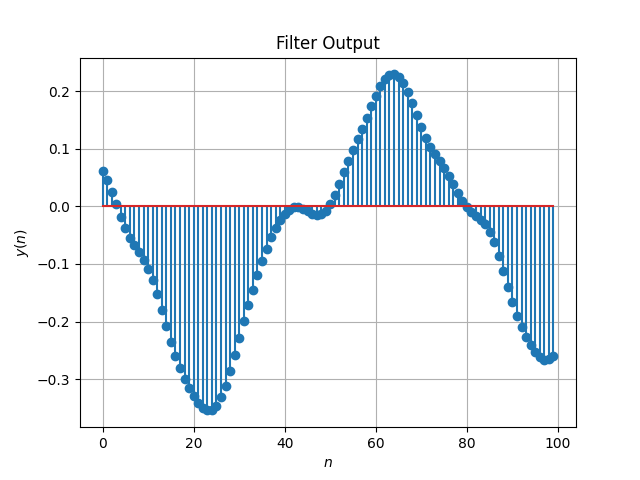
\includegraphics[width=\columnwidth]{./figs/7.2.1.png}
		\caption{Plot of $y(n)$}
		\label{fig-7.2.1}	
	\end{figure}
	
	\begin{figure}[!ht]
		\centering
		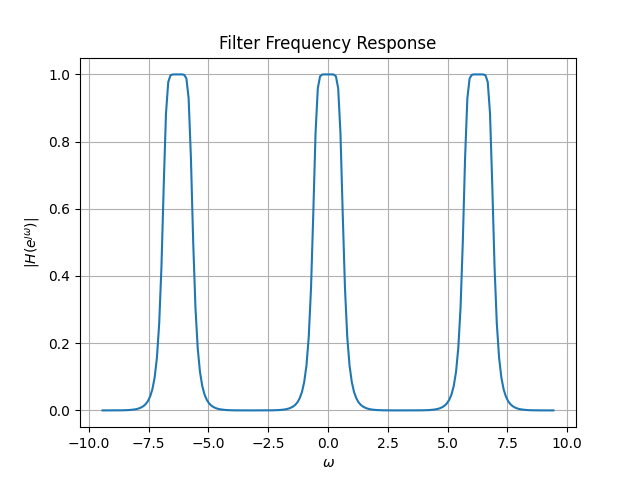
\includegraphics[width=\columnwidth]{./figs/7.2.2.png}
		\caption{Plot of $\abs{H(e^{\j\omega})}$}
		\label{fig-7.2.2}	
	\end{figure}
	
	\begin{figure}[!ht]
		\centering
		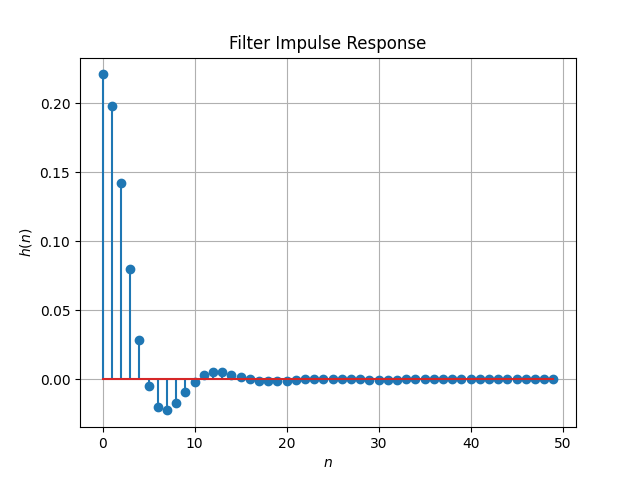
\includegraphics[width=\columnwidth]{./figs/7.2.3.png}
		\caption{Plot of $h(n)$}
		\label{fig-7.2.3}	
	\end{figure}
	
	\item What is the sampling frequency of the input signal?
	
	\solution The sampling frequency of the input signal is \SI{44100}{\hertz} = \SI{44.1}{\kilo\hertz}
	
	\item What is the type, order and cutoff frequency of the above Butterworth filter?
	
	\solution 
	
	Type: low-pass
	
	Order: 4
	
	Cutoff frequency: \SI{4000}{\hertz} = \SI{4}{\kilo\hertz}
	
	\item Modify the code with different input parameters to get the best possible output.
	
	\solution
	
	Order: 10
	
	Cutoff frequency: \SI{3000}{\hertz} = \SI{3}{\kilo\hertz}
	
	\end{enumerate}

\end{document}
